%\section{Guiding Principles and Process of Library Adoption}
%\label{sec:taxonomy}
%\begin{figure*}
%    \centering
%    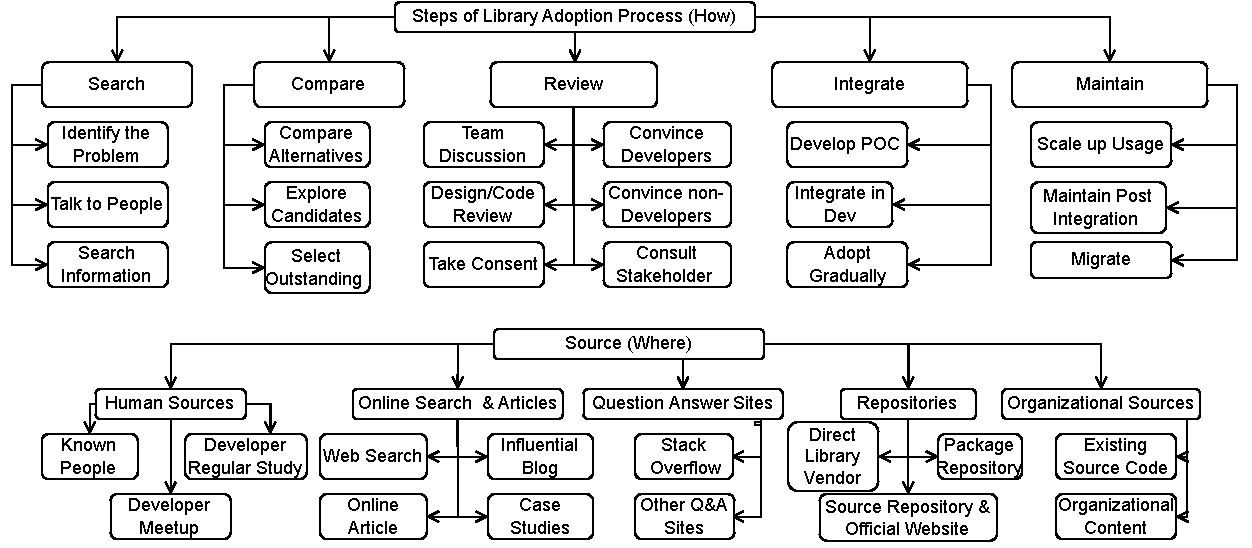
\includegraphics[scale=0.85]{images/process.pdf}
%    \caption{Concepts related with library adoption process and relevant information sources}
%    \label{fig:process}
%\end{figure*}
% Using open coding and constant comparison of \td{24} interviews, we discovered total 83 library adoption concepts. By conducting axial coding, we categorized these concepts into 19 categories under 4 major categories of adoption steps, surrounding conditions, library specific factors, and information sources. Figure \ref{fig:taxonomy} shows the hierarchy of all 83 library adoption concepts. Numbers shown beside the major categories in Figure \ref{fig:taxonomy} refer to the total number of concepts under that category (e.g., 18 concepts under 'steps' category).



\begin{figure*}
    \centering
    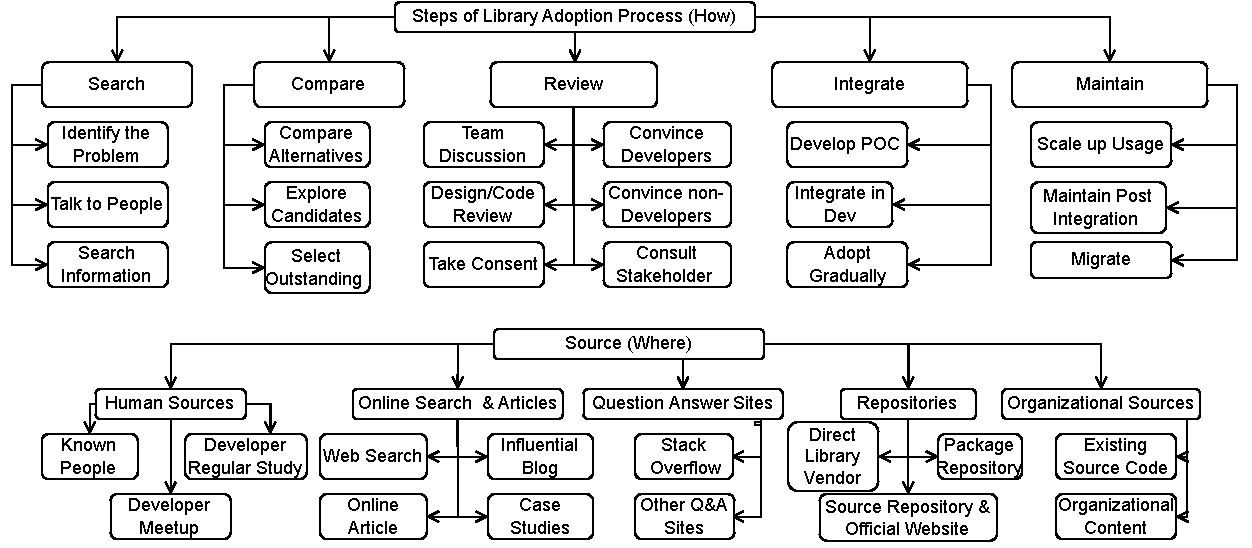
\includegraphics[scale=0.78]{images/process.pdf}
    \caption{Concepts related library adoption process and information sources}
    \label{fig:process}
\end{figure*}

\subsection{Library Adoption Process (P)}\label{sec:phases} 
The adoption of a third-party library consists of five steps, as depicted in Figure~\ref{fig:process}. The steps are: search for library information, compare available libraries, review libraries along with other teammates or teams, integrate the library into the application, and maintain the library through the process of the host application. There were 18 concepts associated with \code{steps of library adoption process} in our code system. Figure \ref{fig:process} shows the relationship between relevant codes and categories for the library selection process and information sources consulted during the process.
%Figure~3 in the Appendix shows the relationship between relevant codes and categories.

\subsubsection{Step 1. Search} \code{Search} entails \code{identifying the problem}, \code{talking to people}, and \code{performing an online search}. 
\subsubsection{Step 2. Compare}
Next, developers \code{compare} available libraries by \code{comparing alternatives}, \code{exploring candidates}, and \code{selecting the outstanding library}. The comparison concept is explained by the interview participant, P15:

\qi{You go to Stack Overflow and you find some articles there that refer to some of the libraries. From there, you go into those libraries spaces and GitHub and then you take a look at it.}{P15} 

% \gias{let's add something from Fig 6}

\subsubsection{Step 3. Review} \code{Review} of the library can involve multiple concepts: \code{team discussion}, \code{design/code review}, \code{consent process}, \code{convince developers}, \code{convince non-developers}, and \code{stakeholder consultation}. Depending on the company size and practices, developers may request approval from dedicated teams who review the security and license issues of third-party libraries: 
\qi{So we have the DevOps team\ldots they have a way to check the security also any vulnerability issue altogether and also if we are actually using it in the proper license.}{P11} 


\subsubsection{Step 4. Integrate} To \code{integrate} a library can also be a gradual process, consisting of \code{proof of concept development}, \code{integration}, and \code{gradual adoption}, as illustrated here:
\qi{[We] do some proof of concept for some libraries. Then for the adoption phase we normally take it slowly, like for example, when we want to introduce Hikary CP instead of Tomcat, we have to apply this library to one or two services, then gradually move to the wide adoption of that library.}{P01} 

\subsubsection{Step 5. Maintain} Finally, to \code{maintain}, developers may \code{scale up usage}, perform \code{post integration maintenance}, and \code{migration}. Once the library has been integrated, developers may need to keep up with the latest versions:

\qi{There is no limit on improvement\ldots You can opt-in for new 
versions or you can ignore the new versions. Usually, major versions might have something which can break your code. But you don’t upgrade without any reason.}{P05}
%\todo{@Minaoar - I took this quote from elsewhere, please replace it if it isn't coded under maintain} \minaoar{looks good}.


\subsection{Information Sources (S)} \label{sec:sources}
Developers seek out information about libraries from five categories of information sources when making an evaluation: \code{human sources}, \code{online search and articles}, \code{question answer sites}, \code{repositories}, and \code{organizational sources} internal to the company. Within these five categories, we identified 15 concepts, whose hierarchical relationship is shown in Figure \ref{fig:process}.

% Of the \code{human sources} available to developers, there are \code{known people}, the developer's \code{regular study}, and \code{developer meetup}. Which sources the developer favors can vary, as illustrated by these two quotes:
% \qi{The first thing is not opinion from other people, rather from developer's daily study. Developers always look for [learning] things, right?}{P01}
% \qi{The very first step before going to searching is I'm reaching out to my colleagues.}{P11}

For \code{online search and articles}, developers can turn to \code{web search}, \code{online article}, \code{influential blog}, and \code{case studies}. Alternately, they may turn to \code{question and answer sites} such as \code{Stack Overflow} or \code{other Q\&A sites}:
\qi{Stack Overflow is a huge resource for seeing what different people recommend\ldots and also seen a lot on things like Quora and Reddit where you say what's the best library for doing X and people will list out a couple of different options there.}{P07}

Another source of information is \code{repositories}, which can consist of the \code{direct library vendor}, \code{package repository}, or \code{source repository and official website}. Finally, developers can turn to internal \code{organizational sources}, namely \code{existing source code} and \code{organizational content}. 
\qi{[We have an] internal GitHub. Then there are internal search engines, also there are some question answers like Stack Overflow\code I think that is true for all these big corporations.}{P02}

One participant shared information about a very unique data source ChatGPT\footnote{\url{https://openai.com/blog/chatgpt}}, a chatbot supported by large-language model:
\qi{One more vector of discovery that I have been lurking with the last few weeks is I'm giving a prompt to ChatGPT or my team is giving a prompt to the copilot, not Googling first, but rather prompting it first and seeing what it gives and then copying and pasting that code into Google and finding out actually what these things actually do and actually are they valid or not. And surprisingly the results of the prompts give you fairly accurate suggestions for the libraries or the APIs that you need to use. I think it's yes I would say probably 70\% of the time it's useful. 30\% of the time they actually give you false names of APIs or functions that actually do not reside in reality or those packages do not exist. }{P16}

\subsection{Conditions Influencing Library Adoption (C)}
\label{sec:conditions}

\begin{figure*}
    \centering
    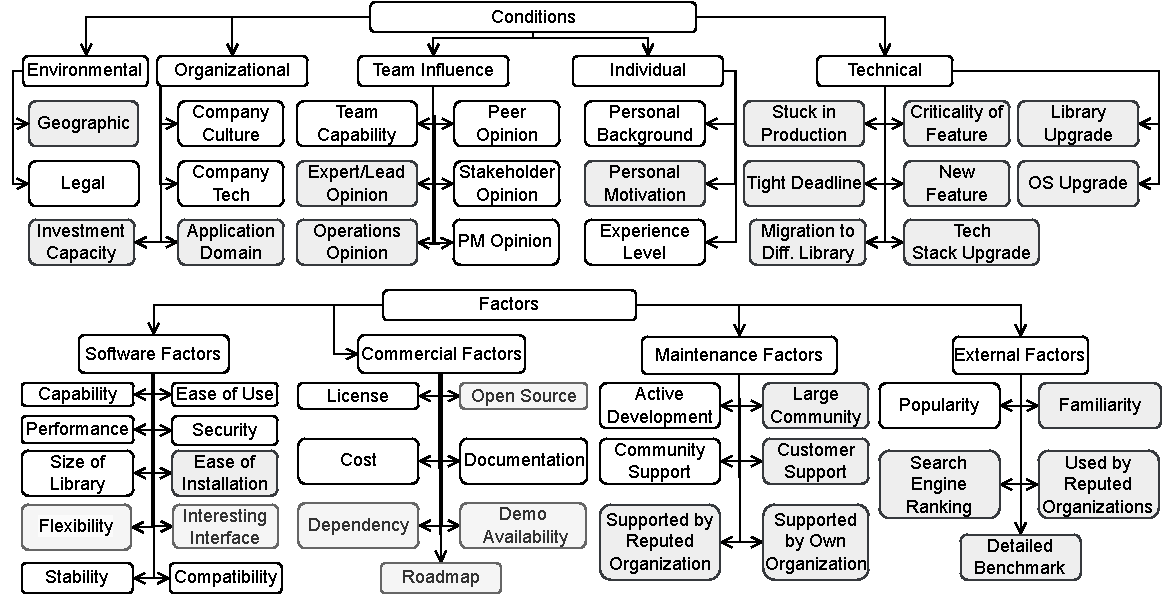
\includegraphics[scale=0.75]{images/conditions.pdf}
    \caption{Factors and conditions influencing adoption process (gray boxes are concepts that are found for the first time in our study)}
    \label{fig:conditions}
\end{figure*} \fig\ref{fig:conditions} summarizes the concepts related to external (environmental) and internal conditions that can influence the library adoption process. 
% Our second research question was ``What conditions and technical factors influence the library adoption process?'' In order to answer this question, we turn to the conditions of library adoption and the factors of library selection criteria.

The library adoption process can be influenced by environmental, organizational, team-specific, individual, and technical scenario-specific conditions and opinions. These conditions affect which guiding principles are most appropriate. In the major category of \code{conditions}, we identified five categories: \code{environmental}, \code{organizational}, \code{team influence}, \code{individual}, and \code{technical}, which are depicted in relation to the process of adoption in Figure~\ref{fig:framework}. There were 23 concepts associated with these categories, as shown in \fig\ref{fig:conditions}.

\code{Environmental} conditions include the \code{geographic} and \code{legal} landscapes. For example, regulatory requirements influence the legal conditions under which the company operates:
\qi{In Germany you have to report a security breach in your company\ldots you have to pay two percent of the revenue if a security breach happens and your data gets leaked.}{P17} 
Geography can influence selection, outside of legal requirements:
\qi{{\ldots} everywhere it's not still functional programming, it's not widely adopted. I recently migrated from Asia to Europe and I never saw this trend widely adopted in our previous companies. But here [in Europe], I've seen a lot of people are very interested in that functional programming paradigms. So, to choose the libraries, maybe their background, their geography, their location, all of these things can have some impact.}{P01}

Organizations can also enforce policies for library selection. Under \code{organizational} conditions, we observed \code{investment capacity}, \code{company culture}, existing \code{company tech}, and \code{application domain}. There can also be a \code{team influence}, based on \code{team capability}, \code{expert/lead opinion}, \code{operations opinion}, \code{peer opinion}, \code{stakeholder opinion}, and \code{product/project manager opinion}. Team capability is demonstrated with the following quote:
\qi{I went for Vue because most of the developers in my company were mostly back-end developers and I found Vue is very back-end developer friendly.}{P04}

\code{Individual} developers can also have personal characteristics which are independent of technology but which influence library selection. These can include \code{personal background}, \code{personal motivation}, and \code{experience level}. An example of personal motivation is:
 \qi{The excitement of trying some new library was also fairly motivating to keep my skills up to date\ldots}{P06} 

 Finally, there can be \code{technical} conditions, namely a severe issue in production (\code{stuck in production}), having a \code{tight deadline}, \code{migration to a different library}, \code{criticality of feature}, \code{new feature}, \code{tech stack upgrade}, \code{library upgrade}, and \code{OS upgrade}. The influence of criticality can be seen here:
\qi{If the feature is too business critical, then it goes through an even more rigorous decision-making process than the other where, for example, you are just trying to choose a library to show an image and crop it. So that is not so business critical.}{P15}


\subsection{Library Selection Factors (F)}
\label{sec:factors}
Based on the selection process and conditions, developers choose the selection factors for a library, as depicted in Figure~\ref{fig:framework}. We identified four categories of \code{factors}: \code{software factors}, \code{commercial factors}, \code{maintenance factors}, and \code{external factors}. Under these, we found 28 concepts, whose relation to the categories is shown in  \fig\ref{fig:conditions}.

In the category of technical \code{software factors}, we see \code{compatibility}, \code{stability}, \code{flexibility}, \code{capability}, \code{security}, \code{performance}, \code{ease of use}, \code{ease of installation}, \code{size of library}, and \code{interesting interface} as concerns. Several of these considerations are provided by P15:
\qi{We have to understand how much memory it is gonna use. How much time does it take to execute? Or how much CPU is gonna use? Is this library compatible with the development environment? How is the thread safety within the library?}{P15}

After technical factors, developers may have to consider \code{commercial factors} such as \code{license}, \code{cost}, \code{dependency}, \code{roadmap}, \code{open source}, \code{documentation}, and \code{demo availability}. An example of the impact of demo availability on the selection process is:
\qi{And one thing I prefer over other GitHub repositories is that if it has a working demo available on the web. For example, if it is a front-end library, then it has a UI. If it's a back-end library, it has some kind of documentation available like Swagger so that I can make a call to the library and see how it works. If some kind of live demo is available, then I feel more confident about it.}{P15}

\code{Maintenance factors} include whether the library source code is under \code{active development}, enjoys \code{community support}, is \code{supported by a reputed organization}, has a \code{large community}, offers \code{customer support}, and is \code{supported by own organization}. 

Finally, \code{external factors} can come into play. These include \code{popularity}, \code{search engine ranking}, \code{familiarity}, \code{used by reputed organizations}, and \code{detailed benchmark}. The following quotations demonstrate how popularity and familiarity affect selection:
\qi{We cannot compare sixty million with one thousand downloads. So this [frequently downloaded] library is obviously a choice.}{P04} 
 \qi{Oftentimes what happens is that the decision or the choice gets influenced by an individual's bias or familiarity or previous experience with one particular product or service}{P08} 

\subsection{Barriers of Library Adoption (B)}
Before being able to integrate a library, there are certain entry barriers that an organization or a developer may try to avoid for considering library usage at all. Such obstacles can be caused by organizational policy, and technology or even by developers' mindset, and experience. We identified a total of seven challenges deriving from three major sources of the organizational culture, individual traits, and industry conditions.
% \subsection{Recommendations}

%\subsubsection{Lack of Organizational Policy}
\nd\bf{\ul{B1. Lack of Supporting Process.}} To manage third party open source libraries, many companies \code{lack supportive process} such as an open source program office. In some cases, organizations may be unclear about what their developers can use and cannot use from third parties, and instead of embracing external libraries, they can be rather rigid: \qi{I was in organizations where they were really so afraid of the legal ramifications of using open source that I had to sit through hours of filling out forms to get approval for each library and so that can be a limiting factor if you're a developer. \textbf{You usually you would spend 100 hours developing something instead of one hour trying to fill out some legal form.}}{P12} 

\nd\bf{\ul{B2. Infrastructural or Technological Limitations}} can also cause difficulty in adopting new libraries. Some organizations \textit{``try to limit the access to the Internet.''}$_{P12}$ and then it's not that easy to install third-party libraries from repositories such as NPM used in Node JS. Also, in some cases, because of the current tech stack of the application, integrating a new library can cause a lot of difficulties. A participant who developed a C++ application in the  Windows environment for over 27 years shared their experience: \qi{C++ libraries are notorious for the amount of work to integrate them, to get them to compile on. Like if the library was designed for Linux, it's really hard to get them actually to compile with Visual Studio, to get your compile flags all right, to get all your dependencies right.}{P18} 

\nd\bf{\ul{B3. Inclusivity Barrier.}} Though library selection is a team decision, sometimes \code{lack of inclusivity} hinders the consideration of all opinions.
Developers seek information from a variety of sources. If the organization does not have a very welcoming, inclusive culture, critical analysis of libraries can be ultimately influenced and driven by outspoken people. 
\qi{Let's say some developers are more vocal, some people are better in writing, and some people are comfortable reading a material before joining a meeting. Moreover, in some cultures, people understand more from the context, and in some other cultures, people understand only from the word that has been spoken. 
In an ideal scenario, every team member can contribute using their preferred communication style - vocal or non-vocal, writing or reading. But in real life, we are a bit diverse from that ideal world where we can make it really inclusive. Oftentimes what happens is that the decision or the choice gets influenced by developers' bias who are more vocal.}{P08}

 \nd\bf{\ul{B4. Lack of a Learning Culture}} across the development team also creates an unbalanced team discussion in situations like library selection. Even when the culture promotes openness, development teams often have few enthusiastic developers who love to explore and whose opinions might have a disproportionate weight in discussions. 
 \qi{there are various types of engineers, some people are very interested in technology careers. So they're always keen to update themselves on the latest technology. Some developers are like regular. They're not too much serious, they're moderate, but they don't go the extra mile. So you have to identify those types of personalities in your team and try to encourage them to get training materials, and read books so that they can also contribute to team discussions.}{P05}


\nd\bf{\ul{B5. Lack of Experience.}} \code{Developers' lack of experience} in software development can allure them to solve some problems by themselves for which there are already robust libraries. They cannot estimate how much work would be needed to implement by themselves: \qi{Then there is the ‘not invented here’ syndrome. So many people think that they can do it better... So you say - oh, I can write just some code doing this, and investing the time to learn the third party library seems like too much investment... And later on, it will turn out that your small project will grow. And then you will basically reimplement whatever it's outside. But at the beginning, it seems that it's easier to do this [implementation] than learning [new library].}{P12}


\nd\bf{\ul{B6. Change-Averse Mindset.}} The analysis also reveals that there can be a \code{mindset of developers} that can hinder them from learning new technologies or libraries and stick to their own development: \qi{So I saw people who were happy to learn and start trying new things and introduce new things [libraries]. And some who were really, really refusing things. And my description is that it's sort of the internal age of the person, so not the external, not your real age, but sort of like it's a mentality thing.}{P12}

\nd\bf{\ul{B7. Lack of Comparison Tools.}} \code{Lack of availability of comparison tools} for libraries make developers confused to choose a library after searching online. With the organization's support, policy, and team's willingness to collaborate and explore libraries, there are always challenges of finding out the appropriate library by going through numerous articles, documents, and reviews online. There still is a lack of guiding tools that can support library selection (or in general, technology selection) by summarizing a large amount of data according to the team's priorities. Developers cannot rely on the existing summarization research outcomes since the detailed reference and quality assurance of those tools still are not considered worthy of industrial usage: \qi{How do people decide? There are like 50 things implementing the same thing. Which one should I use? Then there is analysis paralysis when you have an abundance of choices and then you can't make a choice... I don't see any tools really for that. Maybe there are. I guess there should be or I don't know.}{P12}

\subsection{Decision Patterns of Software Library Adoption (D)}
\label{sec:gp}

All of the concepts of the library adoption process described in this section have complex interactions which we captured in the six \principle. All of the patterns represent an abstract solution to a recurring problem \cite{riehle:2021:pattern}. On the basis of internal and external conditions, certain advantages and disadvantages of libraries become relevant to developers, and they follow a decision pattern accordingly. Thus the \principle\space show interaction among the selection factors, information sources, and the adoption process. 
 \qi{It's not that always you have to choose a library or framework which is technically the best. Rather capabilities of the library and the organization, the domain, the people, the timing, everything influences that decision.}{P01} 

It must be noted that conditions do not come in isolation, and \principle\space also do not activate exclusively. Rather, in practical scenarios, developers are always facing multiple, even conflicting situations, and are balancing between \principle\space to make their final decisions.

% Due to space limitations, we are only able to present some of the guiding principles in depth. All six can be found in the Appendix.

%%%%%%% GP 1
\nd\bf{\ul{D1: Just Do It.}} When developers are concerned primarily with time-to-market or are not that interested in long-term maintenance, they may opt to make use of third-party libraries which are \qqw{F}{easy to use} and \qqw{F}{easy to install}, as illustrated by the following quotes. 

\qi{[The library] makes our life simpler. The application development definitely gets faster by using that.}{P15}
\qi{It was going to solve a particular promotion or something, and it was going to be retired. So usually the long-term maintainability was not a factor.}{P06}

\begin{practice}{1}{Just Do It}
\actor{Developers}
\condition{Faster go to market is critical. Developers rewarded for delivering minimum feature on time.}
\concern{How the developers can meet the deadline with relatively less effort?}
\solution{Use a third-party library that reduces the work load and delivery can be done on time}
\consideration{Easy to use, easy to install, popular, and familiar library.}
\steps{Find libraries, compare them, and choose one according to the consideration. Take support from known people or use search engine or Stack Overflow}
\consequence{Can lead to future maintenance burden such as performance bottleneck or security vulnerability.}
\example{For startups, a lot of it [priority] is just speed to market and how much resources is gonna eat up using any specific library.}{P07}
\end{practice}

% \begin{table}[]
%     \centering
%     \caption{Scenario of GP1: Just Do It}
%     \begin{tabular}{p{1cm}p{6.5cm}}
%          \toprule
%             \textbf{GP} & \textbf{Just Do It} \\ 
%             \midrule
%             Actor(s) & Developers \\ 
%             Context & - Faster go to market is critical for business. Developers are often rewarded for delivering minimum viable product on time.
%             - Developers are in their early career and assume higher satisfaction on faster delivery. \\ 
%             Concern & How the developers can meet the deadline in relatively less effort? \\ 
%             Solution & Use a third-party library that reduces the work load and delivery can be done on time \\ 
%             Consider-ation & The library should be easy to use, easy to install, popular, and even better if developer is already familiar with it. \\ 
%             Steps & Find libraries, compare them, and choose one according to the consideration \\ 
%             Support & Take support from known people to know about such library or use search engine, Stack Overflow \\ 
%             Example Trace in Data & For startups, a lot of it [priority] is just speed to market and how much resources is gonna eat up using any specific library. (P07) \\ 
%          \bottomrule
%     \end{tabular}
%     \label{tab:gp1-scenario}
% \end{table}
 %% Ann: I exclude this one because it is fairly evident (to save space)


%%%%%%%% GP 2
\nd\bf{\ul{D2: Reuse Robust Component.}} Developers working on long-term or complex products prefer to choose \qqw{F}{stable} which are \qqw{F}{actively maintained} for a long period and supported by a \qqw{F}{large community}. The \principle\space is \code{Reuse Robust Component}. Examples of its use are:
 
\qi{%Don't reinvent the wheel. 
I want to use as much as already developed, tested, and robust software in my solution\ldots the main thing is that reusability and having stability in the application inherently out-of-the-box by using a stable, robust library}{P22}
\qi{With a project like ours [C++ code application developed over 27 years], the main time we adopt a library is when it is an implementation of a tech spec. OpenSSL, there's a tech spec for SSL. Here's a whole library that has been carefully implemented against the spec.}{P18}

\begin{practice}{2}{Reuse Robust Component}
\actor{Developers, Senior Developers}
\condition{Mature organization, stable code. Developers concerned of quality, performance \& maintainability.}
\concern{How can the application avoid boiler plate code and follow best design principles?}
\solution{Use a trusted proven third-party library that will keep the code clean and manageable.}
\consideration{Open source, community trusted, stable and high-performing library.}
\steps{Find and compare libraries, review thoroughly by more than one developer. Look into the library's source code repository to analyze the stability, quality of the library, and also consider reputed technical blogs.}
\consequence{Too much analysis and exploration can be an overkill for small features causing delivery delay.}
%\hline
\example{So [this large corporation] as a whole is actually built on the open source libraries that are suitable for our use cases. But that actually has been one of our primary focus as well. If you find a library, use it; only build if you can’t find anything.}{P13}
\end{practice}

% \begin{table}[]
%     \centering
%     \caption{Scenario of GP2: Reuse Robust Component}
%     \begin{tabular}{p{1cm}p{7.5cm}}
%          \toprule
%             \textbf{GP} & \textbf{Reuse Robust Component} \\ 
%             \midrule
%             Actor(s) & Developers, Senior Developers \\ 
%             Context & - Matured organization with stable source code and release pipeline. Application performance and maintainability is a big concern for the team.
%             - Developers with higher experience would be careful about the quality of the application source code. \\ 
%             Concern & How the application can avoid boiler plate code and follow best design principles? \\ 
%             Solution & Use a trusted proven third-party library that will keep the code clean and manageable. \\ 
%             Consider-ation & The library should be open source, trusted by community, stable and provide apppropriate performance metrics required \\ 
%             Steps & Find and compare libraries, review thoroughly by more than one developer. \\ 
%             Support & Look into the library's source code repository to analyze the stability, quality of the library, and also consider reputed technical blogs. \\ 
%             Example Trace in Data & So [this large corporation] as a whole is actually built on the open source libraries that are suitable for our use cases. But that actually has been one of our primary focus as well. If you find a library, use it; only build if you can’t find anything. (P13) \\ 
%          \bottomrule
%     \end{tabular}
%     \label{tab:gp2-scenario}
% \end{table}
 %% Ann: I exclude this one because it is fairly evident (to save space)

%%%%%%% GP 3
% \begin{practice}{1}{Just Do It}
\actor{Developers}
\condition{Faster go to market is critical. Developers rewarded for delivering minimum feature on time.}
\concern{How the developers can meet the deadline with relatively less effort?}
\solution{Use a third-party library that reduces the work load and delivery can be done on time}
\consideration{Easy to use, easy to install, popular, and familiar library.}
\steps{Find libraries, compare them, and choose one according to the consideration. Take support from known people or use search engine or Stack Overflow}
\consequence{Can lead to future maintenance burden such as performance bottleneck or security vulnerability.}
\example{For startups, a lot of it [priority] is just speed to market and how much resources is gonna eat up using any specific library.}{P07}
\end{practice}

% \begin{table}[]
%     \centering
%     \caption{Scenario of GP1: Just Do It}
%     \begin{tabular}{p{1cm}p{6.5cm}}
%          \toprule
%             \textbf{GP} & \textbf{Just Do It} \\ 
%             \midrule
%             Actor(s) & Developers \\ 
%             Context & - Faster go to market is critical for business. Developers are often rewarded for delivering minimum viable product on time.
%             - Developers are in their early career and assume higher satisfaction on faster delivery. \\ 
%             Concern & How the developers can meet the deadline in relatively less effort? \\ 
%             Solution & Use a third-party library that reduces the work load and delivery can be done on time \\ 
%             Consider-ation & The library should be easy to use, easy to install, popular, and even better if developer is already familiar with it. \\ 
%             Steps & Find libraries, compare them, and choose one according to the consideration \\ 
%             Support & Take support from known people to know about such library or use search engine, Stack Overflow \\ 
%             Example Trace in Data & For startups, a lot of it [priority] is just speed to market and how much resources is gonna eat up using any specific library. (P07) \\ 
%          \bottomrule
%     \end{tabular}
%     \label{tab:gp1-scenario}
% \end{table}
 
\nd\bf{\ul{D3: Maximize Flexibility.}} While inspired by the principle of architectural improvement and consistency, architects adopt third-party libraries when absolutely necessary for specifications. Project P18 worked was such an example where they had less than 20 libraries in a two million line source code. Even when they \qqw{P}{integrate} libraries, they would wrap it under their own structure: 

\qi{We will create just a thin wrapper, that ends up looking like the rest of our platform. The simple source file [wrapper API] is protecting the two million lines of code from the idiosyncrasies of this one particular library.}{P18}

\qi{Just go with the smaller libraries that solve a very particular problem so that we have full control. But if we integrate with the framework then we always need to solve with that framework because we cannot go outside of that framework until we completely remove that framework}{P9}
%\vspace{-5mm}
\begin{practice}{3}{Maximize Flexibility} % Was Improve Application Structure
\actor{Developers, Architects}
\condition{Large scale software applications have their own structure which evolved over time and may follow some software design principles. System designers want to use new libraries in a way that improves the application structure, or at least does not deteriorate it.}
\concern{How can the architecture be improved or be protected from unwanted rigidity while using a library?}
\solution{Use a library that just fits right with the application in terms of the size and flexibility. Consider wrapping the third-party library in an API to allow replacement of the library without affecting dependent code.}
\consideration{The library should be flexible and should not be too large in size compared to the system.}
\steps{Find, compare, and review libraries. Conduct design review to assess impact on architecture. Review internal organizational content for design principles.}
\example{The moment you have to bring something in because there are new requirements is the time to assess how you've structured your application and does it still serve you and your customers or the business requirements you have. So that’s the opportunity to look at the structural aspect of the application and make sure you do want to avoid changing it or maybe
it's the time to change it.}{P22}
\end{practice}%\vspace{-4mm}

% \begin{table}[h]
%     \centering
%     %\caption{Scenario of GP3: Maximize Flexibility}
%     \begin{tabular}{p{8.5cm}}%{p{1cm}p{7.5cm}}
%          \toprule
%          \textbf{Guiding Principle 3 - Maximize Flexibility} \\% & \textbf{Improve Application Structure} \\ 
%          \midrule
%             \bf{Actor(s).} Developers, Architects \\ %\midrule 
%             \bf{Condition.} Large scale software applications have their own structure which evolved over time and may follow some software design principles. System designers want to use new libraries in a way that improves the application structure, or at least does not deteriorate it.\\ %\midrule 
%             \bf{Concern.} How can the architecture be improved or be protected from unwanted rigidity while using a library?\\ %\midrule 
%             \bf{Solution.} Use a library that just fits right with the application in terms of the size and flexibility. Consider wrapping the third-party library in an API to allow replacement of the library without affecting dependent code.\\ %\midrule 
%             \bf{Consideration}. The library should be flexible and should not be too large in size compared to the system.\\ %\midrule 
%             \bf{Steps.} Find, compare, and review libraries. Conduct design review to assess impact on architecture. Review internal organizational content for design principles.\\ %\midrule 
%             \bf{Example}. \emph{``The moment you have to bring something in because there are new requirements is the time to assess how you've structured your application and does it still serve you and your customers or the business requirements you have. So that’s the opportunity to look at the structural aspect of the application and make sure you do want to avoid changing it or maybe it's the time to change it."}{P22} \\ 

%          \bottomrule
%     \end{tabular}
%     \label{tab:gp3-scenario}
% \end{table}
 


%%\vspace{-5mm}
\begin{practice}{3}{Maximize Flexibility} % Was Improve Application Structure
\actor{Developers, Architects}
\condition{Large scale software applications have their own structure which evolved over time and may follow some software design principles. System designers want to use new libraries in a way that improves the application structure, or at least does not deteriorate it.}
\concern{How can the architecture be improved or be protected from unwanted rigidity while using a library?}
\solution{Use a library that just fits right with the application in terms of the size and flexibility. Consider wrapping the third-party library in an API to allow replacement of the library without affecting dependent code.}
\consideration{The library should be flexible and should not be too large in size compared to the system.}
\steps{Find, compare, and review libraries. Conduct design review to assess impact on architecture. Review internal organizational content for design principles.}
\example{The moment you have to bring something in because there are new requirements is the time to assess how you've structured your application and does it still serve you and your customers or the business requirements you have. So that’s the opportunity to look at the structural aspect of the application and make sure you do want to avoid changing it or maybe
it's the time to change it.}{P22}
\end{practice}%\vspace{-4mm}

% \begin{table}[h]
%     \centering
%     %\caption{Scenario of GP3: Maximize Flexibility}
%     \begin{tabular}{p{8.5cm}}%{p{1cm}p{7.5cm}}
%          \toprule
%          \textbf{Guiding Principle 3 - Maximize Flexibility} \\% & \textbf{Improve Application Structure} \\ 
%          \midrule
%             \bf{Actor(s).} Developers, Architects \\ %\midrule 
%             \bf{Condition.} Large scale software applications have their own structure which evolved over time and may follow some software design principles. System designers want to use new libraries in a way that improves the application structure, or at least does not deteriorate it.\\ %\midrule 
%             \bf{Concern.} How can the architecture be improved or be protected from unwanted rigidity while using a library?\\ %\midrule 
%             \bf{Solution.} Use a library that just fits right with the application in terms of the size and flexibility. Consider wrapping the third-party library in an API to allow replacement of the library without affecting dependent code.\\ %\midrule 
%             \bf{Consideration}. The library should be flexible and should not be too large in size compared to the system.\\ %\midrule 
%             \bf{Steps.} Find, compare, and review libraries. Conduct design review to assess impact on architecture. Review internal organizational content for design principles.\\ %\midrule 
%             \bf{Example}. \emph{``The moment you have to bring something in because there are new requirements is the time to assess how you've structured your application and does it still serve you and your customers or the business requirements you have. So that’s the opportunity to look at the structural aspect of the application and make sure you do want to avoid changing it or maybe it's the time to change it."}{P22} \\ 

%          \bottomrule
%     \end{tabular}
%     \label{tab:gp3-scenario}
% \end{table}

%% GP 4
 %% Ann: I include this one because it is not something most people consider
\nd\bf{\ul{D4: Empower the Team.}} 
%\vspace{-5mm}
\begin{practice}{4}{Empower the Team}
\actor{Developers, Tech Leaders}
\condition{Strong company culture to promote transferable skill and provide learning space for developers. 
%Tech leaders may care more for their team's capacity, limitations, and motivations.
The development team may have limitations or strengths in certain technologies. }
\concern{Does the library fit well within the capability of the dev team? Will it provide any transferable skills?}
\solution{Use a library appreciated by the developers}
\consideration{Well documented, popular, easy to use library with customer support.}
\steps{Besides finding a library that fits well with the technology, thoroughly discuss with developers about their opinion and acceptance of the library. Look into official documentation of the library.}
\consequence{May compromise the optimum technology for dev team's limitation. Can keep teams motivated.}
\example{So looking at community popularity helps because then it helps to hire people. It helps to retain people. They like to use technologies that are transferable.}{P19}
\end{practice}%\vspace{-4mm}


% \begin{table}[]
%     \centering
%     \caption{Scenario of GP4: Empower the Team}
%     \begin{tabular}{p{1cm}p{7.5cm}}
%          \toprule
%             \textbf{GP} & \textbf{Empower the Team} \\ 
%             \midrule
%             Actor(s) & Developers, Tech Leaders \\ 
%             Context & - Some organizations may have strong company culture to improve development skill set or for providing comfortable learning space for developers. 
%             - Tech leaders may care more for their team's capacity, limiatation, and motivation.
%             - Development team may have limitation or strength in certain technology  \\ 
%             Concern & Does the library fit well with the capability of the development team? Will it provide them any transferable skill? \\ 
%             Solution & Use a library that is appreciated by the developers \\ 
%             Consider-ation & Library should be well documented, should be community popular so that developers can easily adopt and can refer in future. Also it can have customer support in case developers needs extra help. \\ 
%             Steps & Besides finding a library that fits well with the technology, thoroughly discuss with developers about their opinion and acceptance of the library. \\ 
%             Support & Look into official documentation of the library for documentation and support issues. \\ 
%             Example Trace in Data & So looking at community popularity helps because then you can it helps to hire people. It helps to retain people. They like to use technologies that are transferable (P19) \\ 
%          \bottomrule
%     \end{tabular}
%     \label{tab:gp4-scenario}
% \end{table}

Adopting third-party libraries also empowers the development teams. Open-source libraries provide developers with working experience with popular development components to acquire transferable knowledge whereas proprietary solutions developed internally can create bottlenecks: 
\qi{When you move to use something that's an open source third-party solution, it's well documented, suddenly an entire team of people can help address a problem, and your speed to fixing something goes from multiple days or weeks to hours. And you empower the whole team rather than an [internal] specialist who can't go on vacation because if she does, sorry, you're waiting.}{P22}

 When following this empowering \principle, developers often consider \qqw{C}{peer opinions} during the library \qqw{P}{review} phase: 
  \qi{I'm not taking a decision for myself. Also, there are seniors in every organization who are more experienced and they may have some opinions on it.}{P01}
 \qi{Let's say, I proposed one library from my previous work. And then I have to explain it to the team members.}{P10}




%% GP 5
\nd\bf{\ul{D5: Ensure Compliance.}} Third-party libraries can come with licensing issues, privacy concerns, or security vulnerabilities.
However, not all development teams equally consider the impact of compliance issues. \qqw{C}{Legal environment} of the organization or their customers are the primary driver for compliance principle: 
\qi{Since we work with people from Europe, the UK, the US, and other areas and they have a very strong data security policy, we have to be confident that they're secure well.}{P04} 
\qi{So there are libraries who advertise that they are already GDPR \cite{website:gdpr} compliant or FedRAMP \cite{website:fedramp} compliant. So those kinds of libraries are always preferred over libraries that don't have a clear signal.}{P19} 

\begin{practice}{5}{Ensure Compliance}
\actor{Developers, Information Security Experts, Legal Experts, Open Source Program Office}
\condition{Because of regulatory compliance or for company culture, some organizations will be more cautious about using third-party libraries for legal, security, and privacy reasons. 
Developers will often have little technical expertise on such specialized issues.
Sometimes small or early stage companies may even ignore the importance of compliance issues.
A few application domains such as health, finance, media are also more regulated and require organizational policies for ensuring compliance.}
\concern{Will there be any penalty or legal complication arising from using a third-party library? How to protect the organization?}
\solution{Use a library which is compliant with the application security standards and legal requirements}
\consideration{The license of the library should be compatible with the business and license of the target software. The security and privacy concerns should be clarified and well taken care of by the library contributors.}
\steps{Reach out to specialists in the organization for taking their expert consent before adopting the library. See the license and security declarations in the library documentation in the source code or package repository.}
\example{We had a very bad experience with this. With the legacy system, we were using so many different libraries and there is a licensing issue and we had to replace half of the library. Otherwise we had to pay lots of money. So that's why we are now very, very concerned about adding any external library, because if we don’t comply with the license, it will be a legal problem.}{P09}
\end{practice}

% \begin{table}[]
%     \centering
%     \caption{Scenario of GP5: Ensure Compliance}
%     \begin{tabular}{p{1cm}p{7.5cm}}
%          \toprule
%             \textbf{GP} & \textbf{Ensure Compliance} \\ 
%             \midrule
%             Actor(s) & Developers, Information Security Experts, Legal Experts, Open Source Program Office \\ 
%             Context & - Because of regulatory compliance or for company culture, some organizations will be more cautious about using third-party libraries for legal, security, and privacy reasons. 
%             - Developers will often have little technical expertise on such speialized issues
%             - Sometimes small or early stage companies may even ignore the importance of compliance issues
%             - Few application domains such as health, finance, media are also more regulated and require organizational policies for ensuring compliance. \\ 
%             Concern & Will there be any penalty or legal complication arising from using a third-party library? How to protect the organization? \\ 
%             Solution & Use a library which is compliant with the application security standards and legal requirements \\ 
%             Consider-ation & License of the library should be compatible with the business and license of the target software. The security and privacy concerns should be clarified and well take care of by the library contributors. \\ 
%             Steps & Reach out to specialists in the organization for taking their expert consent before adopting the library. \\ 
%             Support & See the license and security declarations in the library documentation in the source code or package repository. \\ 
%             Example Trace in Data & we had a very bad experience with this. With the legacy system, we were using so many different libraries and there is a licensing issue and we had to replace half of the library. Otherwise we had to pay lots of money. So that’s why we are now very, very concerned about adding any external library, because if we don’t comply with the license, it will be a legal problem. (P09) \\ 
%          \bottomrule
%     \end{tabular}
%     \label{tab:gp5-scenario}
% \end{table}
 %% Ann: I exclude this one because it is fairly evident (to save space)

%% GP 6
\nd\bf{\ul{D6: Maintain Continuous Stability.}} Aside from compliance issues, the biggest risk of using a third-party library is that the library won't be maintained.

\qi{If the contributors are gone in those third-party libraries repositories, suddenly the whole production application is broken}{P10} 

To protect themselves from abandonment and stability risks, developers look for libraries where a \qqw{F}{large community} and contributors are involved. To \qqw{P}{search information} about \qqw{F}{active development}, they check \qqw{S}{source repositories}: 
\qi{We have to check whether this library maintenance is active or not. We can determine that by checking their GitHub repository when the last push was given?}{P04} 

\begin{practice}{6}{Maintain Continuous Stability}
\actor{Developers, DevOps}
\condition{Some software applications are developed and maintained for long term. A third-party library used in such a product can have bugs or vulnerabilities that need to be fixed. Sometimes, the contributors of the library may not continue to fix bugs or improve with new features. Sometimes libraries may not have backwards compatibility and when developers upgrade, their existing system can break.}
\concern{How will developers ensure that a library is well maintained in foreseeable future and that they can keep using the library without breaking their application?}
\solution{Use a library with good history of maintenance and prepare to continuously upgrade the library in future}
\consideration{Selected libraries should be actively maintained by contributors, supported by reputed organizations, and have larger community.}
\steps{Analyze the maintenance and issue history of the library to assess the active development practices or the library. Establish a process for software bill of materials to document all third-party library dependencies and their upgrade plan in conjunction with DevOps teams. Look into source code commit and issue history from source repository and download usage trend from package repository.}
\example{When we integrated the updated version our whole interface broke. And we had to change a lot of code, all the interceptors, interfaces, everything\ldots This maintenance is quite hard. It's actually a full time work to always keep updated, to always stay updated.}{P14}
\end{practice}

% \begin{table}[]
%     \centering
%     \caption{Scenario of GP6: Maintain Continuous Stability}
%     \begin{tabular}{p{1cm}p{7.5cm}}
%          \toprule
%             \textbf{GP} & \textbf{Maintain Continuous Stability} \\
%             \midrule
%             Actor(s) & Developers, DevOps \\ 
%             Context & - Some software applications are developed and maintained for long term. A third-party library used in such a product can have bugs or vulnerabilities that need to be fixed. Sometimes, the contributors of the library may not continue to fix bugs or improve with new features. Sometimes libraries may not have backwards compatibility and when developers upgrade, their existing system can break. \\ 
%             Concern & How developers will ensure that a library is well maintained in foreseeable future and can keep using the library without breaking their application? \\ 
%             Solution & Use a library with good history of maintenance and prepare to continuously upgrade the library in future \\ 
%             Consider-ation & Selected libraries should be actively maintained by contributors, supported by reputed organizations, and have larger community. \\ 
%             Steps & Analyze the maintenance and issue history of the library to assess the active development practices or the library. Establish a process for software bill of materials to document all third-party library dependencies and their upgrade plan in conjunction with DevOps teams. \\ 
%             Support & Look into source code commit and issue history from source repository and download usage trend from package repository. \\ 
%             Example Trace in Data & when we integrated the updated version our whole interface broke. And we had to change a lot of code, all the interceptors, interfaces, everything... This maintenance is quite hard. It’s actually a full time work to always keep updated, to always stay updated. (P14) \\ 
%          \bottomrule
%     \end{tabular}
%     \label{tab:gp6-scenario}
% \end{table}
 %% Ann - excluded to save space


% During the theoretical integration of our study, the six guiding principles emerged from the benefits and baggage of libraries - why developers want to use a library and why they still remain cautious to use a library.











